\section{Обзор}

Существуют различные подходы к автоматическому управлению памятью, 
каждый из которых имеет свои преимущества и недостатки
~\cite{book:jones1996garbage,book:jones2011garbage}. 
В данной главе будут рассмотрены основные алгоритмы сборки мусора, 
а также подходы к автоматическому управлению памятью, актуальные в 
контексте C++. 
Кроме того, представлен обзор существующих решений задачи
сборки мусора для языка C++. 


\subsection{Обзор алгоритмов сборки мусора}

Различают два принципиально различных подхода к автоматическому управлению памятью: 
\emph{подсчёт ссылок} (\emph{reference counting}) и \emph{трассирующая сборка мусора} 
(\emph{tracing garbage collection}). 
Существует множество различных разновидностей трассирующей сборки мусора, 
мы рассмотрим две из них: \emph{сжимающую} (\emph{compacting garbage collection}) и 
\emph{инкрементальную} (\emph{incremental garbage collection}).


\subsubsection{Подсчёт ссылок}
\label{sec:ref_cnt}

Одним из наиболее простых методов автоматического управления памятью является 
\emph{подсчёт ссылок}. 
С каждым объектом, выделенным в куче, связывается целое число ~---~ \emph{счётчик ссылок}. 
Изначально, значение счётчика инициализируется единицей. 
При копировании указателя на объект его счётчик увеличивается на единицу, 
а при удалении указателя ~---~ уменьшается на единицу. 
Когда значение счётчика падает до нуля, объект может быть удалён. 

К достоинствам данного подхода можно отнести то, что он прост для понимания, 
легко реализуем, и, кроме того, момент освобождения памяти строго детерминирован~---
как только в программе не остаётся ссылок на определённый объект, 
занимаемая им память может быть освобождена и переиспользована. 
Однако данный подход обладает рядом недостатков.

\begin{enumerate}
\item 
	Поддержка счётчика ссылок накладывает дополнительные накладные расходы на все 
	операции с указателями.
\item 
	Имеется вероятность \emph{лавинного освобождения памяти}, т.е. ситуации, 
	при которой уничтожение одной ссылки на ``корень'' структуры данных приводит 
	к цепному освобождению целой области памяти, вызывая тем самым 
	\emph{непредсказуемую} по продолжительности паузу в процессе исполнения программы.
\item 
	\emph{Циклические структуры данных} (множества объектов, содержащих взаимные ссылки) 
	не могут быть корректно обработаны без модификации алгоритма 
	(наличие таких структур приводит к утечке памяти).
\end{enumerate}

Ясно, что второй недостаток прямо связан с детерминированным моментом освобождения памяти, 
и попытка преодолеть его также приведёт и к потере этого преимущества. 
Для решения третьей проблемы были предложены различные модификации алгоритма, 
однако они либо достаточно сложны и вычислительно трудоёмки, либо перекладывают 
ответственность за разрешение циклических ссылок на программиста \cite{book:jones1996garbage}. 
Например, может быть введён новый примитив ~---~ \emph{невладеющий указатель} (weak pointer). 
Невладеющий указатель не участвует в подсчёте ссылок. 
Используя этот указатель для хранения ссылок, замыкающих цикл, можно предотвратить 
утечку памяти.


\subsubsection{Трассирующая сборка мусора}
Принципиально другой подход к сборке мусора основан на использовании критерия 
доступности объекта. 
\emph{Доступность} определяется индуктивно, а именно, область памяти называется 
\emph{доступной}, если либо указатель на неё принадлежит корневому множеству, 
либо существует указатель на неё из другой области памяти, являющейся доступной. 
\emph{Корневое множество} представляет собой множество априори доступных объектов. 
Конкретное определение корневого множества зависит от языка программирования и среды 
времени выполнения. 
Зачастую, корневым множеством является множество указателей, расположенных в 
регистрах, на стеке и в статической области памяти. 
Все объекты, которые не являются доступными, объявляются \emph{мусором}. 
Сборщики мусора, использующие данный подход, называются \emph{трассирующими}. 
Инвариантом данного подхода является то, что память, занимаемая мусором, 
в любой момент может быть безопасно освобождена. 
Тем самым доступность является эвристическим приближением понятия \emph{используемости}. 
Заметим, что проблема используемости памяти неразрешима\footnote{Может быть показано, что 
проблема используемости памяти сводится к проблеме остановки: \\
\url{https://en.wikipedia.org/wiki/Tracing\_garbage\_collection\#Reacha}\\{bility\_of\_an\_object}}. 

Базовым алгоритмом трассирующий сборки мусора является алгоритм 
\emph{пометить и освободить} (\emph{mark-and-sweep}). 
Сборщик мусора обходит граф достижимых объектов, начиная с корневого множества, 
помечая все достижимые объекты как живые (для хранения метки с каждым объектом 
связывается специальный бит). 
Затем, память из-под всех непомеченных объектов освобождается. 
Компонент, выполняющий пометку и освобождение, называют \emph{сборщиком}, 
а компонент, модифицирующий память и запрашивающий её выделение, ~---~ \emph{мутатором}. 

Ввиду того, что мутатор может модифицировать объекты и менять структуру графа 
достижимых объектов, перед запуском маркировки и освобождения он должнен быть остановлен. 
Алгоритмы сборки мусора, требующие полной остановки работы приложения на время своей работы, 
известны как \emph{алгоритмы с полной остановкой мира} (\emph{stop-the-world algorithms}).

Трассирующие сборщики мусора можно разделить на два класса:
\begin{itemize}
\item 
	\emph{точные} (\emph{precise}/\emph{accurate}) сборщики мусора, 
	которые способны обнаружить все недоступные объекты;
\item 
	\emph{консервативные} (\emph{conservative}) ~---~ сборщики мусора, 
	не являющиеся точными.
\end{itemize}

Для точной трассирующей сборки мусора необходимо выполнение следуюших условий:
\begin{itemize}
\item 
	возможность построения корневого множества;
\item 
	возможность определить все указатели из любого объекта на другие области 
	управляемой памяти.
\end{itemize}

Часто, в силу особенности языка программирования, устройства среды 
времени выполнения или по другим специфическим причинам, выполнение этих 
условий невозможно. 
В таком случае, без наложения дополнительных ограничений на использование 
языковых 
средств, возможна только консервативная сборка мусора. 
При этом используются различные эвристические методы построения корневого множества 
или идентификации ячейки памяти как указателя. 
Это приводит к тому, что для каждого консервативного сборщика мусора существует целый класс 
программ, на которых выбранные эвристики работают недостаточно хорошо\cite{boehm1993space}. 
Следствием этого могут стать длительные задержки в работе сборщика или же полное исчерпание 
памяти.


\subsubsection{Сжимающая сборка мусора}
\label{sec:two-finger-compact}

\emph{Сжимающая сборка} (\emph{compacting garbage collection})~---~это разновидность 
трассирующей сборки, предназначенная для решения проблемы \emph{фрагментации памяти}. 
\emph{Фрагментацией} называется ситуация, при которой в куче выделено большое число блоков, 
не образующих непрерывную область памяти. 
В таком случае попытка выделения объекта большого размера может закончиться неудачей, 
несмотря на то, что суммарного количества свободной памяти вполне достаточно для 
удовлетворения запроса. 

Алгоритм сжимающей сборки \emph{``пометить и сжать''} 
(\emph{mark-and-compact}) 
после этапа маркировки запускает процедуру сжатия кучи. 
Все живые объекты перемещаются на место непереживших сборку, образуя тем самым непрерывные 
области памяти, а программные указатели на них перенаправляются на новое 
расположение объектов (\emph{pointer forwarding}). 

Для сжатия кучи могут применяться различные алгоритмы. 
Базовым алгоритмом сжатия кучи является \emph{двухпальцевый алгоритм} 
(\emph{two-finger-compact}). 
Мы рассмотрим одну из модификаций двухпальцевого алгоритма, которая может применяться 
для сжатия области памяти, содержащей объекты фиксированного размера. 
Заметим, что существуют и другие вариации алгоритма, позволяющие сжимать кучу с объектами 
произвольного размера, но мы не рассматриваем их, так как в текущей версии библиотеки они 
не применяются. 
Алгоритм поддерживает два указателя: указатель на свободный объект и 
указатель на перемещаемый объект. 
Первый указатель инициализируется адресом начала сжимаемой области памяти, 
а второй~--- адресом конца. 
Затем выполняется поиск очередного свободного блока (первым указателем) и 
очередного перемещаемого объекта (вторым указателем). 
Память, занимаемая перемещаемым объектом, копируется в свободный блок, 
а на её место записывается так называемый \emph{перемещающий указатель} 
(\emph{forward pointer}), указатель на новое расположение объекта. 
Перемещающий указатель затем используется в фазе модификации указателей на 
перемещённые объекты. 
Алгоритм повторяет вышеописанный процесс, пока указатель на свободный блок 
меньше указателя на перемещаемый объект. 


\subsubsection{Инкрементальная параллельная маркировка}
\label{sec:inc_marking}

Алгоритмы, позволяющие чередовать работу коллектора и мутатора называются 
\emph{инкрементальными}. 
Инкрементальные алгоритмы разбивают цикл сборки мусора на несколько частей, 
тем самым размывая паузы, вызываемые работой сборщика мусора, по исполнению программы.
При этом снижается время каждой конкретной паузы мутатора, 
и уменьшаются задержки в работе приложения, вызванные остановкой на сборку 
мусора. 
Однако инкрементальная сборка, как правило, привносит накладные расходы, 
так что суммарное время работы приложения может увеличиться по сравнению 
с подходами с полной остановкой мутатора. 
Алгоритмы сборки, способные выполнять большую часть своей работы 
(часто, всю работу лишь за исключением сканирования корневого множества) 
по сборке мусора одновременно с работой мутатора, называются 
\emph{почти паралелльными} (\emph{mostly-concurrent}).  

Далее мы рассмотрим модификацию алгоритма ``пометить и сжать'', 
которая позволяет 
производить маркировку без остановки мутатора, остановка мира необходима только для 
сканирования корневого множества, а также на этапе сжатия кучи. 
Чтобы рассмотреть такую модификацию, введём несколько определений. 
Разделим все объекты на три класса: 

\begin{itemize}
\item 
	\emph{белые}~---~объекты, которые еще не были сканированы сборщиком мусора;
\item 
	\emph{серые}~---~ объекты, которые были помечены сборщиком, но не все поля 
	которого были просканированы;
\item 
	\emph{чёрные}~---~объекты, которые были помечены сборщиком, и все их поля 
	были просканированы.
\end{itemize}

При инкрементальной маркировке может возникнуть ситуация, в которой чёрный объект 
будет содержать ссылку на белый. 
После завершения маркировки белый объект будет освобождён, а чёрный будет хранить 
некорректный указатель. 
Такая ситуация может возникнуть при выполнении одновременно двух условий:
\begin{itemize}
\item 
	мутатор сохраняет указатель на белый объект в чёрном;
\item 
	не существует серого объекта, такого, что существует путь от него до рассматриваемого 
	белого объекта.
\end{itemize}

\begin{figure}[h!]
\centering
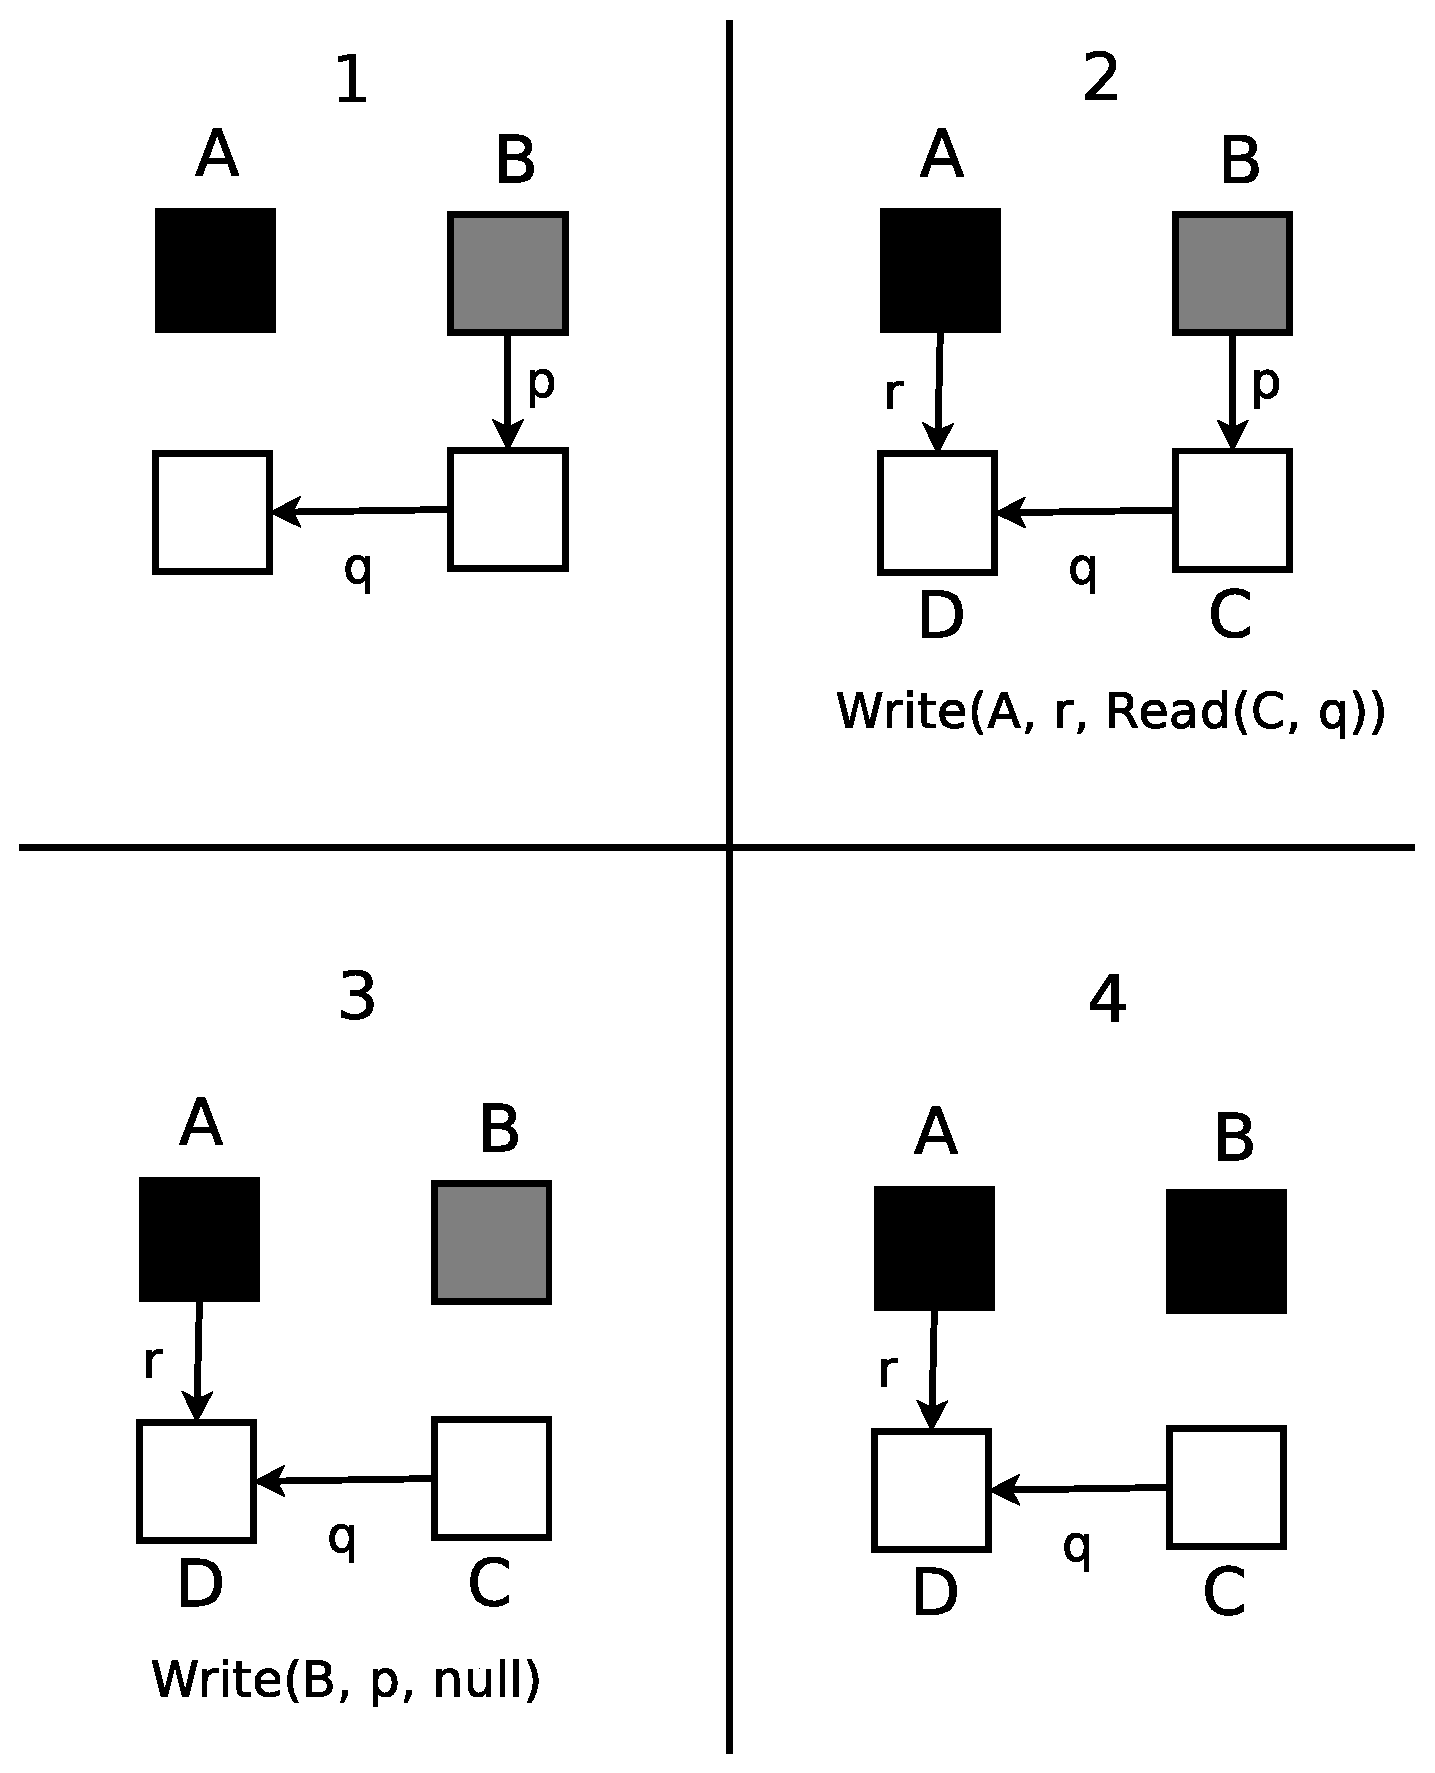
\includegraphics[width=0.4\linewidth]{Moiseenko/images/inc_marking.eps}
\caption{Пример ошибочной ситуации}
\label{fig:inc_marking}
\end{figure}

Рассмотрим конкретный пример. На Рис.~\ref{fig:inc_marking} показано, как последовательность 
действий сборщика и мутатора может привести к подобному некорректному состоянию кучи. 
В начальном состоянии куча содержит четыре объекта~--- чёрный объект \code{A}, 
серый объект \code{B} и два белых объекта \code{C} и \code{D}.
При этом имеются ссылки \code{p} и \code{q} из объекта \code{B} в \code{С} и из 
\code{C} в \code{D}, соответственно. 
Затем мутатор создаёт ещё одну ссылку \code{r}~--- из \code{A} в \code{D}. 
Хотя теперь появилась ссылка из чёрного объекта в белый (первое условие выполнено), 
объект D всё ещё достижим из серого объекта B (второе условие нарушено), следовательно 
рано или поздно объект \code{D} будет просканирован сборщиком. 
Однако затем мутатор удаляет ссылку из \code{B} в \code{C}, что приводит к 
выполнению сразу двух условий, и возникновению некорректного состояния.

Для предотвращения ошибочной ситуации сборщик и мутатор должны поддерживать один из двух 
инвариантов.

\begin{enumerate}
\item 
	\emph{Слабый трёхцветный инвариант} (\emph{weak tricolor invariant}): для любого 
	белого объекта, на который указывает чёрный объект, существует серый объект, такой, 
	что существует путь от этого серого объекта до рассматриваемого белого.
\item 
	\emph{Сильный трёхцветный инвариант} (\emph{strong tricolor invariant}): не существует 
	чёрных объектов, указывающих на белые.
\end{enumerate}

Для поддержки инвариантов могут быть использованы \emph{барьеры чтения} или 
\emph{барьеры записи}. 
Барьером чтения называется перехват чтения полей белого объекта, барьером записи ~---~ 
прехват записи ссылок на белый объект в чёрный. 
Заметим, что последовательность инструкций, реализующая барьер, выполняется при каждой 
операции чтения/записи во время фазы маркировки объектов, накладывая тем самым дополнительные 
расходы на время выполнения работы операций с указателями. 
Барьеры могут быть реализованы либо программно, либо с помощью аппаратной поддержки, 
либо с использованием функций операционной системы. 
Далее мы будем рассматривать только барьер записи, так как именно он используется в нашей 
работе. 
Этот выбор обоснован тем, что операции записи, как правило, выполняются реже, 
следовательно, и барьер записи вызывается реже, а значит и накладные расходы 
меньше. 
Существуют различные реализации барьеров записи, каждая из которых 
поддерживает один из двух упомянутых выше инвариантов. 
Приведём псевдокод барьера записи, впервые предложенного в работе~\cite{dijkstra1978fly}:

\begin{minipage}{\linewidth}
% \begin{lstlisting}[caption={Барьер записи Дейкстры}, label={code:write_barrier}]
\begin{lstlisting}[caption={Dijkstra Barier}, label={code:write_barrier}]
Write(src, field, ptr):
    src->field = ptr
    Shade(ptr)
    
Shade(ptr):
    if white(ptr)
        colour(ptr) = grey
\end{lstlisting}
\end{minipage}

Заметим, что для корректной работы сборщика мусора необходимо, чтобы обе операции в функции 
\emph{Write} были атомарны. 


\subsection{Сборка мусора в C++}

Как уже отмечалось, язык C++ разрабатывался с расчётом на использование 
ручного управления памятью. 
Поддержка сборки мусора не была изачально добавлена разработчиками языка и по сей день 
не включена в стандарт\footnote{ISO/IEC, Working Draft, Standard for Programming Language C++,
\url{http://www.open-std.org/jtc1/sc22/wg21/docs/papers/2014}\\{/n4296.pdf}}. 
В \cite{boehm2007transparent} было упомянуто три подхода для добавления сборки мусора в 
язык, подробно описанных ниже.

\begin{enumerate}
\item 
	Подход, основанный на \emph{умных указателях} (\emph{smart pointer})~--- 
	объектах специального класса, оборачивающих сырые (\emph{raw pointer}) указатели и добавляющие 
	к ним некоторую функциональность. 
	Зачастую, умные указатели используются для реализации подсчёта ссылок, 
	однако могут быть реализованы и другие алгоритмы автоматического управления памятью.
\item 
	Подход, основанный на введении нового типа данных для хранения указателей на 
	управляемые объекты. 
	Экземпляры этого нового типа имеют более бедный интерфейс по сравнению с обычными 
	указателями, например, запрещена адресная арифметика. Существенное отличие от 
	предыдущего подхода~--- использование поддержки со стороны компилятора. 
	Хорошим примером реализации данного подхода служит нестандартное расширение 
	C++/CLI\footnote{C++/CLI Language Specification,
	\url{http://www.ecma-international.}\\{org/publications/files/ECMA-ST/ECMA-372.pdf}}, разработанное компанией Microsoft.
\item 
	\emph{Прозрачная} (\emph{transparent}) сборка мусора. Этот подход подразумевает 
	использование обычных указателей с возможностью переиспользования памяти. 
	Примером реализации прозрачной сборки является сборщик мусора 
	Бёма-Демерса-Вайзера\footnote{Официальный сайт проекта: http://www.hboehm.info/gc/}.
\end{enumerate}

В языках C/C++ указатели хранятся в памяти как целые числа. 
Иными словами, представление указателей в памяти никак не отличается от представления 
других примитивных типов данных. 
Из сказанного выше ясно, что без наложения дополнительных ограничений или введения новых 
типов данных для хранения указателей, точная сборка невозможна в C/C++. 
Поэтому, третий подход подразумевает использование консервативного сборщика. 
Также стоит отметить, что в рамках третьего подхода затруднительно реализовать 
сжимающий сборщик мусора.


\subsection{Существующие решения}
\label{sec:cpp_solutions}

Рассмотрим более подробно существующие решения для автоматического управления памятью в C++. 

Шаблонный класс \code{shared\_ptr<T>} из стандартной библиотеки C++--11
~---~ умный указатель, реализующий алгоритм подсчёта ссылок для автоматического управления 
памятью. 
\emph{Умный указатель} (\emph{smart pointer})~--- это класс--декоратор, добавляющий некоторую 
функциональность к обычному интерфейсу указателей. Умные указатели используют целый ряд 
языковых возможностей C++ (в том числе новые возможности, добавленные в стандарте С++11), 
такие как переопределение операторов, семантика перемещения (move semantics) и другие, 
для предоставления удобного и интуитивно понятного интерфейса. 
Также, как правило, используется идиома RAII (Resource Acquisition Is Initialization). 
В самом общем смысле, использование этой идиомы позволяет связывать некоторые операции с 
конструированием и уничтожением объекта. 
Для этого создается специальный класс--обёртка над каким-либо ресурсом, в конструкторе этого 
класса вызываются функции, связанные с инициализацией ресурса, а в деструкторе ~---~ с 
освобождением ресурса. 
Например, конструктор \code{shared\_ptr<T>} инициализирует контрольный блок (специальный 
объект, хранящий счётчик ссылок и указатель на функцию зачистки), а деструктор выполняет 
проверку счётчика ссылок и при необходимости освобождает память, занятую объектом и его 
контрольным блоком.

Как отмечалось в разделе~\ref{sec:ref_cnt}, один из главных недостатков наивного подсчёта 
ссылок ~---~ некорректная обработка циклических ссылок. 
Для преодоления этой проблемы программисту предлагается использовать объекты класса 
\code{weak\_ptr<T>}~--- невладеющие указатели. 
Перекладывание задачи по обработке циклических ссылок на пользователя библиотеки приводит 
к возможности возникновения в программе труднообнаружимых ошибок.

Расширение C++/CLI было разработано компанией Microsoft для возможности интеграции программ 
на C++ с программной платформой .Net. .Net использует общеязыковую среду исполнения 
(Common Language Runtime), управление памятью в которой происходит при помощи трассирующего 
сборщика мусора. 
Для того чтобы обеспечить совместимость C++ с CLR в язык необходимо было добавить поддержку 
управляемых объектов, что и было сделано. 
Для хранения указателей на управляемые объекты был введён новый тип данных 
T\textasciicircum, который, однако, предоставляет более бедный интерфейс по сравнению с 
обычными указателями. 
Подход C++/CLI позволяет совмещать ручное и автоматическое управление памятью, сборка 
мусора является точной и сжимающей. Но скомпилировать программы, написанные на C++/CLI, 
можно только специальным компилятором, поддерживающим нестандартные расширения языка.

Среди консервативных сборщиков мусора для С++ наиболее популярным является уже 
упоминавшийся сборщик BoehmGC. 
Одна из главных целей, которую преследовали разработчики этого сборщика ~---~ 
возможность использования сборки мусора в существующих проектах с минимальной 
модификацией исходного кода и минимальными ограничениями на использование языковых 
возможностей. 
BoehmGC использует алгоритм ``пометить и освободить''. 
Для выделения памяти программист должен использовать функцию \code{GC\_malloc}, 
которая сохраняет необходимую для сборщика метаинформацию. 
BoehmGC используется в таких проектах, как Mono, Portable.NET, 
GNU Compiler for Java и других. 
Также он может быть использован для поиска утечек памяти, и в таком качестве он 
применяется в продуктах компании Mozilla. 
BoehmGC не требует поддержки от компилятора. 
К его недостаткам можно отнести консервативность и отсутствие поддержки сжимающей 
сборки мусора.


\section{Анализ предыдущей версии библиотеки}
\label{sec:old_lib}

В рамках проекта лаборатории JetBrains была реализована библиотека сборки мусора для 
языка C++ \cite{book:precisegc_berezun,book:precisegc_samofalov,book:precisegc_secr}. 
Реализованный сборщик мусора является почти точным, копирующим, не требует поддержки 
от компилятора и позволяет совмещать ручное и автоматическое управление памятью. 
Используется модификация алгоритма ``пометить и сжать'', 
мутатор останавливается на время маркировки и сжатия. 
От пользователя библиотеки ожидается выполнение некоторых соглашений, необходимых для 
корректной работы сборщика. 
Библиотека может быть скомпилирована только компилятором gcc для 64 битной архитектуры 
и операционной системы Linux, однако в дальнейшем возможен перенос на другие платформы, 
который потребует переработки лишь небольшой части платформозависимого кода.

Далее в данной главе будет приведён детальный обзор реализации предыдущей версии 
библиотеки, будут рассмотрены интерфейс библиотеки, реализация корневого множества и 
кучи, структура метаинформации, необходимой для сборки мусора, используемый алгоритм 
остановки мира и механизм взаимодействия с сырыми указателями.

\subsubsection{Интерфейс}
Библиотека основана на подходе, использующем умные указатели для поддержки 
автоматического управления памятью. 
Пользователю предоставляется шаблонный класс \code{gc\_ptr<T>} для хранения 
умных указателей и шаблонная функция \code{gc\_new<T>} для создания 
управляемый объектов в куче. 
Класс \code{gc\_ptr<T>} определяет конструктор по умолчанию, конструктор от нулевого указателя 
(\code{nullptr}), конструктор копирования, оператор присваивания, оператор доступа к члену 
класса (\code{operator->()}), оператор разыменования (\code{operator*()}), оператор 
преобразования в тип \code{bool} (для проверки, является ли указатель нулевым), 
метод \code{reset} для обнуления указателя. 
Пример использования примитивов библиотеки приводится в листинге~\ref{code:lib_example}. 

\begin{figure}[h!]
\begin{lstlisting}[language={c++}, caption={Пример использования примитивов библиотеки}, 
label={code:lib_example}]
struct Node {
    Node(const gc_ptr<Node>& left, 
         const gc_ptr<Node>& right)
        : left_(left)
        , right_(right)
    {}
    
    gc_ptr<Node> left_;
    gc_ptr<Node> right_;
};
...
gc_ptr<Node> a, b;
...
gc_ptr<Node> c = gc_new<Node>(a, b);
\end{lstlisting}
\end{figure}

\subsubsection{Корневое множество}
Корневым множеством полагается множество указателей на управляемые объекты на стеке и 
в статической памяти. 
Корневое множество хранится в памяти как список указателей на объекты \code{gc\_ptr}, 
являющиеся корнями. 
Чтобы снизить издержки на синхронизацию, каждый поток имеет свой экземпляр списка 
указателей на корни. 
Корневое множество поддерживается в консистентном состоянии при помощи \code{gc\_new} и 
конструктора \code{gc\_ptr}. 
В конструкторе \code{gc\_ptr} проверяется уровень вложенности вызовов \code{gc\_new}, и 
если он равен нулю, то создаваемый указатель является корнем. 
Новые корни добавляются в голову списка, при удалении корня список также просматривается, 
начиная с головы. 
Это связано с тем, что в C++ порядок вызова деструкторов почти всегда обратен порядку 
вызова конструкторов (временные объекты могут нарушать это предположение), поэтому такая 
оптимизация позволяет в большинстве случаев быстро добавлять и удалять корни.

\subsubsection{Метаинформация}
Для того, чтобы сборщик имел возможность построить граф достижимых объектов, каждый объект 
должен содержать дополнительную метаинформацию, позволяющую определить, указатели на какие 
объекты он содержит. 
В нашей библиотеке используются два типа метаинформации: метаинформация класса и 
метаинформация объекта. 
Метаинформация класса хранит размер экземпляра данного класса и список смещений \code{gc\_ptr}, 
содержащихся в экземпляре класса, относительно начала объекта. 
Метаинформация класса создается один раз при первом выделении объекта данного класса в 
управляемой куче. 
С каждым объектом, выделенным в управляемой куче, связана метаинформация объекта. 
Она хранится в куче сразу после самого объекта. 
Метаинформация объекта содержит указатель на метаинформацию класса, указатель на начало 
объекта и количество экземпляров класса внутри управляемого 
объекта\footnote{Под объектом в данном случае понимается не экземпляр какого-либо класса, 
а область памяти в управляемой куче.} (для поддержки массивов). 
Метаинформация создается и поддерживается с помощью специального протокола взаимодействия 
\code{gc\_new} и конструктора \code{gc\_ptr}, подробное описание которого может быть найдено 
в работе \cite{book:precisegc_secr}.

\subsubsection{Куча}
\label{sec:heap}
Для хранения управляемых объектов используется собственная реализация кучи. 
Для выделения объектов больших (больше 4096 байт) и маленьких размеров используются 
различные стратегии. 
Куча для объектов маленьких размеров представляет собой набор пулов 
(segregated storage\footnote{\url{http://www.memorymanagement.org/glossary/s.html\#term-simple}\\
{segregated-storage}}), 
каждый из которых обслуживает объекты определённого размера. 
Адресное пространство кучи разделено на страницы, по умолчанию размер страницы равен 4096 байт. 
Размеры объектов являются степенями двойки от 32 (минимальный размер управляемого объекта) до 
4096 байт. 
Пул выделяет память блоками размера, кратного размеру страницы, с помощью системного вызова 
\code{mmap}. 
Затем этот блок делится на подблоки равного размера. 
С каждым блоком также связывается дескриптор, хранящий два битовых массива:
массив битов маркировки (\code{mark\_bits}) и массив битов закрепления (\code{pin\_bits}) ~---~ а также другую метаинформацию. 
Блоки индексируются с помощью двух-трёх уровневого сильноветвящегося дерева. 
Дерево индексации позволяет по указателю на управляемый объект за константное время 
определить связанный с ним дескриптор и соответствующие биты маркировки и закрепления, 
а также по произвольному указателю определить, является ли объект, на который он указывает, 
управляемым. 
Большие объекты выравниваются по размеру страницы и выделяются напрямую с помощью системного 
вызова \code{mmap}. 
С ними также связывается дескриптор, который хранит размер объекта а также 
бит маркировки и бит закрепления.

\subsubsection{Остановка мира}
На стадии сжатия и освобождения кучи все потоки приложения приостанавливаются. 
Однако поток может быть приостановлен не в любой момент, а только когда соблюдаются 
определенные инварианты, необходимые для корректной работы сборщика. 
К примеру, предположим, что сборщик мусора решит приостановить поток мутатора, в то время 
как он выделяет новый блок памяти из кучи. 
Поток может быть приостановлен в середине этой операции, и куча окажется в неконсистентном 
состоянии.
    
\emph{Безопасной точкой} называется такое состояние мутатора, в котором он может быть 
приостановлен сборщиком. 
Если сборщик мусора имеет поддержку со стороны компилятора, как правило, именно компилятор 
расставляет безопасные точки в пользовательском коде. 
То есть компилятор вставляет последовательность инструкций, которая проверяет, была ли 
запрошена сборка мусора, и останавливает поток, если необходимо. 
Как уже упоминалось, наша библиотека не имеет поддержки компилятора. 
Поэтому, безопасные точки в предыдущей версии были вручную расставлены в некоторых 
примитивах библиотеки, например, в функции \code{gc\_new}. 
Такое решение имеет существенный недостаток: если какой-либо поток редко использует 
примитивы библиотеки, он не сможет быть остановлен сборщиком. 
Сборка мусора не может быть начата, пока все потоки мутатора не будут приостановлены. 
Таким образом, пользователь библиотеки мог столкнуться с ситуацией, при которой сборка 
мусора никогда бы не была вызвана. 
Для преодоления этой проблемы в данной работе был предложен новый алгоритм остановки мира, 
описанный в разделе~\ref{sec:stw}.

Стоит также отметить, что для остановки мира, как в старой, так и в новой реализации, 
необходимо поддерживать список активных потоков. 
Для поддержки этого списка была реализована обёртка над библиотекой \code{std::thread}. 
Пользователь библиотеки должен использовать шаблонную функцию \code{create\_managed\_thread} 
для создания нового управляемого потока. 
Эта функцию принимает функтор и набор аргументов, создаёт новый поток, регистрирует его в 
списке активных потоков, вызывает функтор на переданных аргументах и затем удаляет поток из 
списка. 
Функция \code{create\_managed\_thread} возвращает экземпляр класса \code{std::thread}. 
Заметим, что пользователь не обязан регистрировать все потоки приложения, достаточно лишь тех, 
что будут обращаться к управляемой куче. 
Таким образом, в программе одновременно могут существовать неуправляемые и управляемые потоки, 
причём в фазе остановки мира приостановлены будут только последние. 

\subsubsection{Преобразование управляемого указателя в сырой}
Для хранения управляемых указателей пользователь библиотеки должен использовать объекты 
класса \code{gc\_ptr}. 
Однако иногда может понадобиться получить сырой\footnote{\emph{Сырым} 
указателем называется обычный указатель C/C++ вида T*, 
где T~---~тип объекта.} 
указатель на управляемый объект (например, для передачи такого указателя 
в функцию сторонней библиотеки, 
не знающей о существовании сборки мусора). 
Отметим также, что некоторые указатели в программе не могут быть 
умными~\cite{book:jones1996garbage}, например, указатель \code{this}. 
Проиллюстрируем это нижеследующим примером.

\begin{minipage}{\linewidth}
\begin{lstlisting}[language={c++}, caption={Неявное разыменование 
	\code{gc\_ptr}}, label={code:this_example}]
struct A {
    int x;
    int y;
    void f() {
        x = 0;
        y = 42;
    }
}

gc_ptr<A> a = gc_new<A>();
a->f();
\end{lstlisting}
\end{minipage}

В данном примере при вызове метода \code{f()} сырой указатель на объект 
\code{a} (\code{this}) будет неявно сохранен на стеке. 
Если между строками 5 и 6 работа приложения будет остановлена сборщиком мусора, а объект 
\code{a} будет перемещен, то после возобновления исполнения на стеке окажется некорректный 
указатель, после чего поведения программы становится неопределенным 
(\emph{undefined behaviour}). 

Для предотвращения этой ситуации в предыдущей версии библиотеки разыменованные управляемые 
указатели заносились в хэш-таблицу разыменованных указателей. 
Перед запуском сборки мусора просматривались стеки потоков. 
Указатели на стеке, содержащиеся в хеш-таблице, считались корнями. 
Также у объектов, на которые они указывали, выставлялся бит закрепления. 
Наличие этого бита говорило сборщику, что указанный объект не может быть перемещён. 
Момент, когда закрепление может быть снято, не отслеживался точно. 
Все указатели из хэш-таблицы, которые не были найдены на стеке, удалялилсь из неё перед 
возобновлением работы мутатора.

Так как сборщик мусора использовал консервативный обход стека для идентификации 
разыменованных указателей, строго говоря, он не являлся точным. 
Была возможна ситуация, при которой не оставалось указателей на объект, и тем не менее 
занимаемая им память не освобождалась. 
Поэтому предыдущая версия сборщика мусора являлась \emph{почти-точной} (\emph{mostly-precise}). 
В данной работе предложен новый механизм преобразования управляемых указателей в сырые 
указатели, который возвращает сборщику свойство точности и позволяет точно отслеживать 
момент, когда закрепление может быть снято.
